\chapappendix

\section{The MaNGA Instrumental Line-Spread Function}
\label{chap1:apdx:lsf}

The line-spread function of a spectrograph will introduce an additional ``blur" in the spectral dimension, beyond that produced by astrophysical velocity dispersion. Additionally, the width of the (presumed-Gaussian) resolution element varies across the instrument by nearly a factor of two. This has the potential to severely hamper the quality and reliability of the SFH fits. For example, assuming a constant kernel width across the full MaNGA wavelength range will:

\begin{itemize}
    \item Artificially increase measured velocity dispersions. This effect will be a pervasive and systematic bias, and will not simply increase the width of the velocity dispersion PDF.
    \item Potentially introduce other systematics related to how certain absorption lines reflect different stellar populations.
\end{itemize}

A more subtle effect results from the process of de-redshifting a spectrum into the rest frame. The width of the (observed-frame) LSF, in pixels, will be modified by a factor of $\frac{1}{1 + z}$, such that higher-redshift galaxies will seem to experience less instrumental blurring in the rest-frame. If all observed galaxies were assumed to have a redshift of zero, then this would be a $sim 10\%$ effect; however, by assuming a fiducial redshift of .04, this effect becomes less important, on average. A slight redshift bias may persist, which could be solved by producing many (redshift-dependent) PCA solutions. In practice, repeated (expensive) LSF convolutions and SVD operations defeats the speed gains of the PCA parameter fitting, and so a single fiducial redshift is deemed sufficient.

\section{Constructing synthetic observations using held-out test data}
\label{chap1:apdx:fakedata}

Here we address PCA's ability to recover properties of synthetic spectra, derived from known SFHs and stellar properties. We use held-out test data generated identically to the CSP model library to construct synthetic datacubes, with similar statistical properties to observed MaNGA galaxies, as described in Appendix \ref{chap1:apdx:fakedata}. The process is as follows:

\begin{enumerate}
    \itemsep0em
    \item Obtain a full-resolution model spectrum, along with the properties used to generate it (``truth")
    \item Read in MaNGA DRP and DAP products, which will be used to generate the remaining galaxy properties such as cosmological redshift and velocity field, without having to model them explicitly.
    \item Convolve model spectrum with fiducial instrument dispersion (interpolated to the correct wavelength grid), after adjusting for the cosmological redshift of the source \citep{cappellari_17}
    \item Redshift the model according to the velocity field from the DAP products (making a high-resolution cube in the observed frame)
    \item Scale each spaxel according to the total $r$-band flux map from the DRP products
    \item Down-sample the observed-frame model spectra onto the MaNGA instrument's wavelength grid
    \item Add noise according to the inverse-variance arrays from the DRP products
    \item Mask additional spaxels where velocity field is not well-defined
    \item Write out synthetic DRP \& DAP datacubes and ``ground-truth" values for the parameters PCA will estimate.    
\end{enumerate}

The PCA parameter estimation method is then used in the same manner as on the science data. One example is shown below in Figure \ref{fig:full_diag_fake}

\begin{figure}
    \centering
    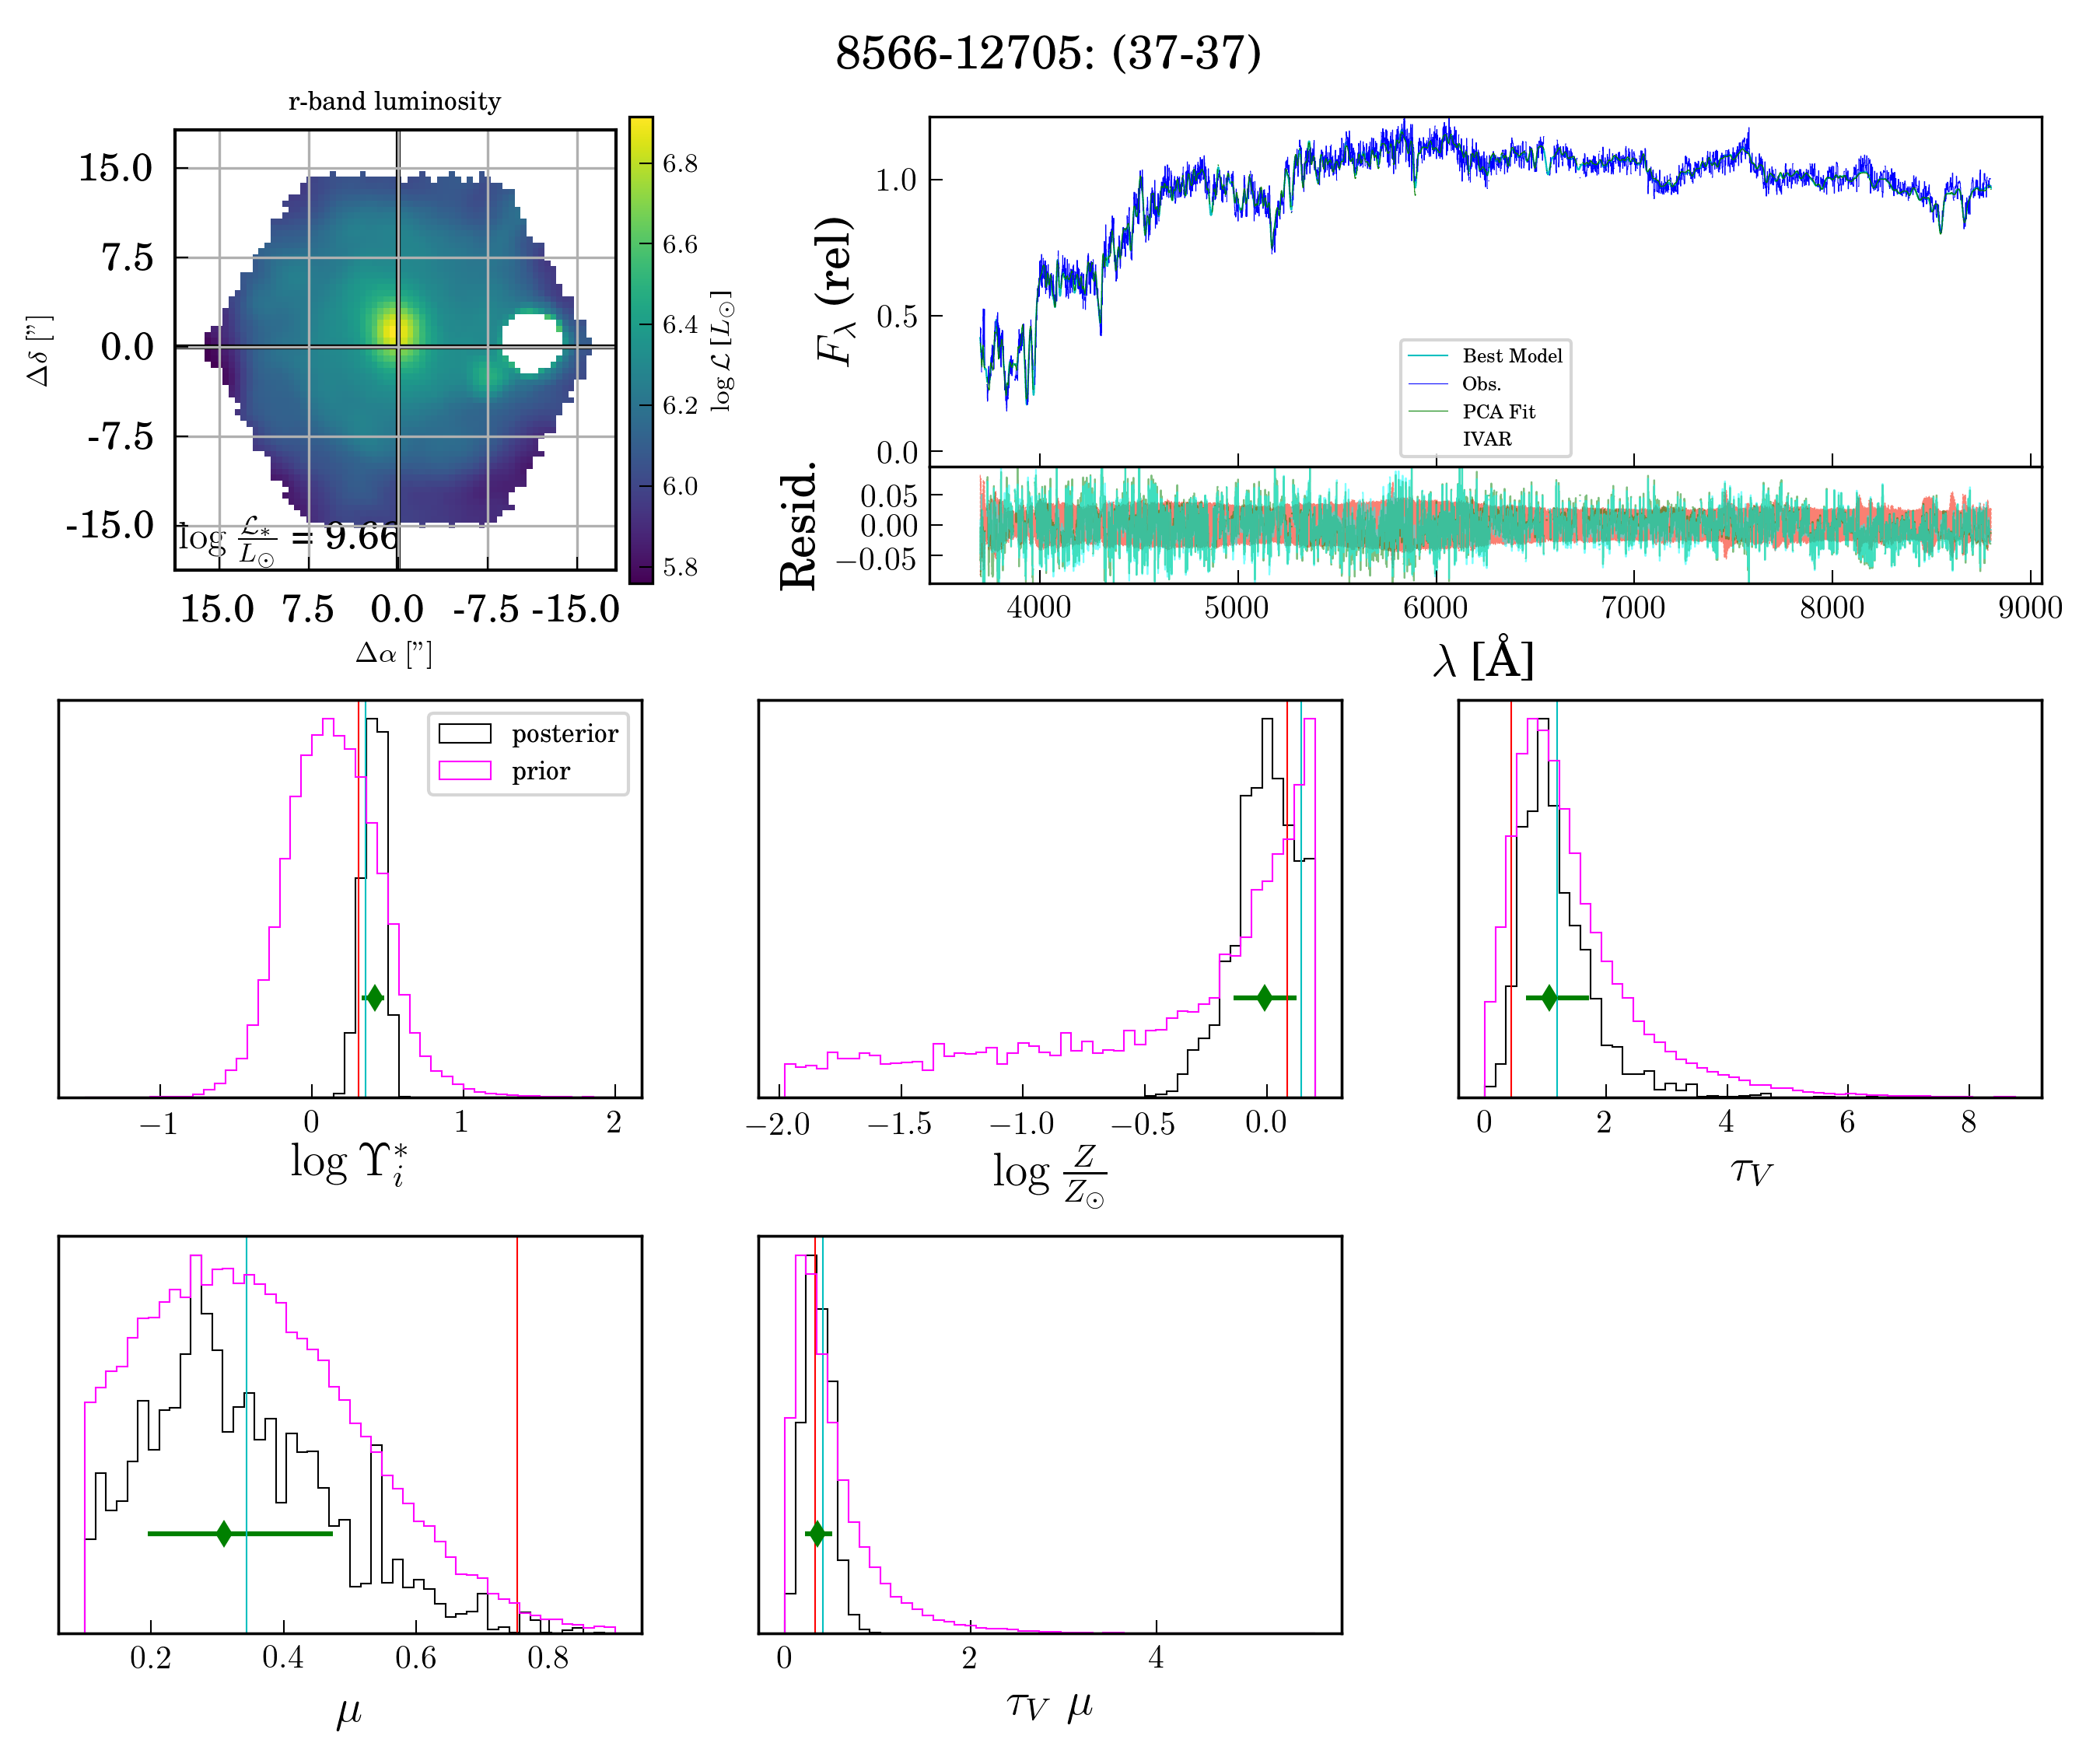
\includegraphics[width=\textwidth,height=\textheight,keepaspectratio]{8566-12705_fulldiag_37-37_mock}
    \caption[Full diagnostic figure for synthetic data based on the test galaxy 8566-12705]{Full diagnostic figure for synthetic data based on the test galaxy 8566-12705. Same format as Figure \ref{fig:sample_fit}, with the addition of a vertical, red line on the parameter histograms denoting the actual value of the parameter.}
    \label{fig:full_diag_fake}
\end{figure}

\section{Statement of Work}
\label{chap1:apdx:statement_of_work}

Here are briefly outlined the contributions of all listed authors for this publication, in order of their listing in the journal article.

\begin{itemize}
	\item \textbf{Zachary J. Pace}: Led development of the SFH modelling, the PC downprojection, the tests of inference accuracy, the software pipeline (including rollout at the University of Utah); also led the writing of this manuscript.
	\item \textbf{Christy Tremonti}: Provided input on the SFH model set, and suggested tests of the methodology; proofreading and revisions.
	\item \textbf{Yanmei Chen:} Advised the lead author during summer appointment as NSF EASPSI Fellow at Nanjing University (Nanjing, China) during Summer 2016.
	\item \textbf{Adam Schaefer:} Aided in devising tests of the methodology; proofreading and revisions.
	\item \textbf{Matthew Bershady:} Aided in understanding the stellar models, particularly the role of the Calcium triplet; proofreading and revisions.
	\item \textbf{Remaining authors} (Kyle Westfall, M\'{e}d\'{e}ric Boqien, Kate Rowlands, Brett Andrews, Joel Brownstein, Niv Drory, David Wake): Proofreading and revisions; inclusion as Sloan Digital Sky Surveys Architects due to contributions to hardware, administration, survey science or software.
\end{itemize}

\endchapappendix